\subsection{Wyniki bez indeksów}

\begin{figure}[H]
    \centering
    
\includegraphics[width=1.0\textwidth]{charts/explain/explain_scan_changes_small.png}
    \caption{Zmiany typów skanów -- wolumen small, bez indeksów}
\end{figure}

\begin{figure}[H]
    \centering
    
\includegraphics[width=1.0\textwidth]{charts/explain/explain_scan_changes_medium.png}
    \caption{Zmiany typów skanów -- wolumen medium, bez indeksów}
\end{figure}

\begin{figure}[H]
    \centering
    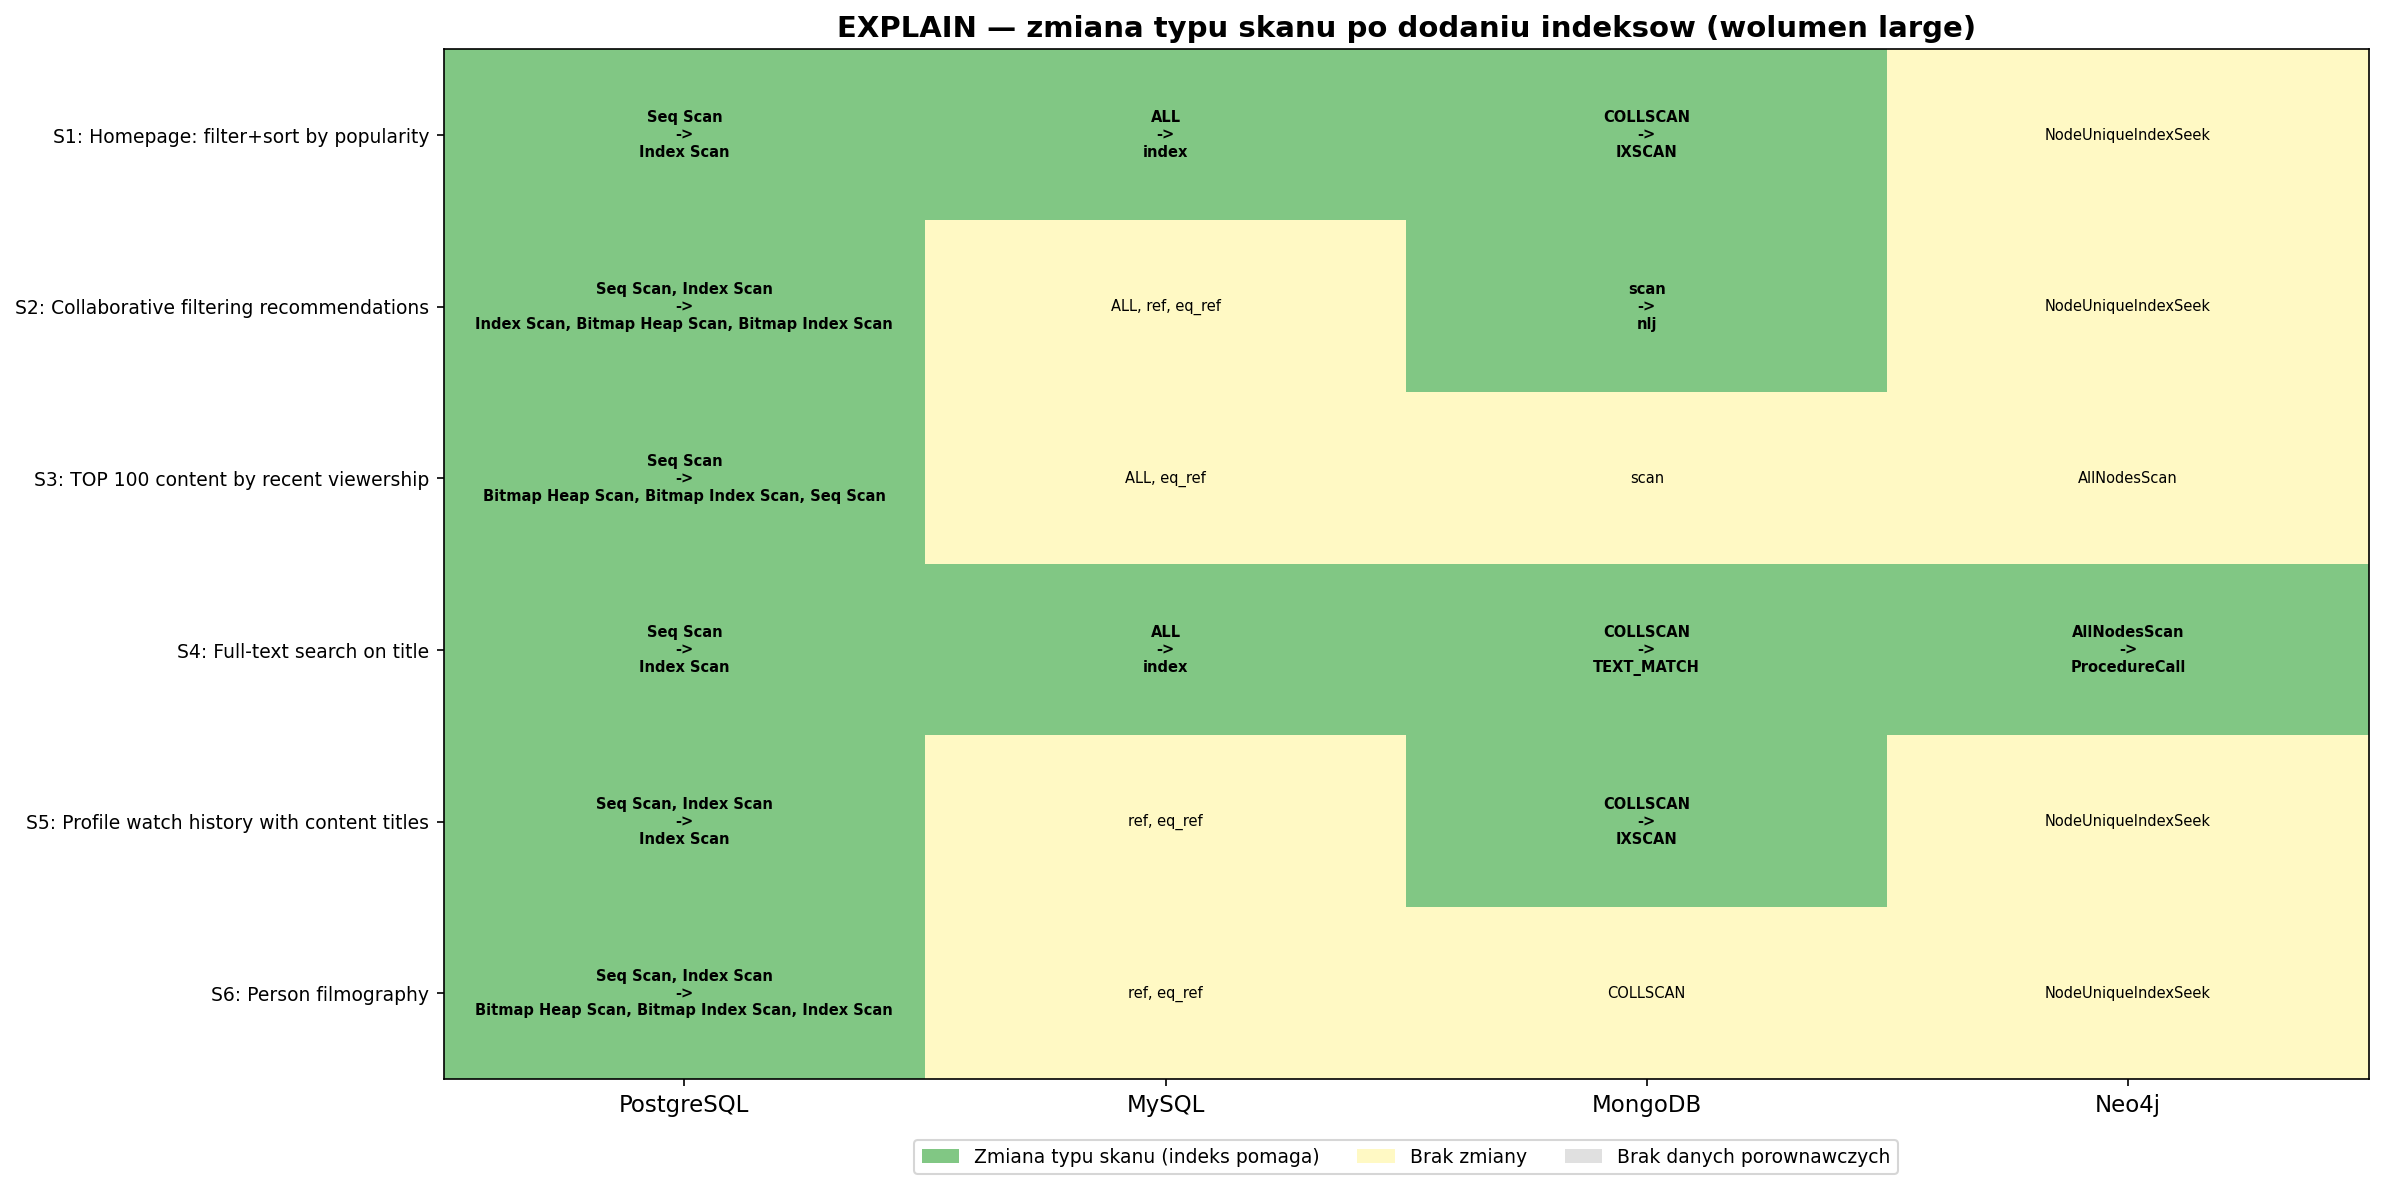
\includegraphics[width=1.0\textwidth]{charts/explain/explain_scan_changes_large.png}
    \caption{Zmiany typów skanów -- wolumen large, bez indeksów}
\end{figure}

\begin{figure}[H]
    \centering
    
\includegraphics[width=1.0\textwidth]{charts/explain/explain_rows_examined_small.png}
    \caption{Liczba przejrzanych wierszy -- wolumen small, bez indeksów}
\end{figure}

\begin{figure}[H]
    \centering
    
\includegraphics[width=1.0\textwidth]{charts/explain/explain_rows_examined_medium.png}
    \caption{Liczba przejrzanych wierszy -- wolumen medium, bez indeksów}
\end{figure}

\begin{figure}[H]
    \centering
    
\includegraphics[width=1.0\textwidth]{charts/explain/explain_rows_examined_large.png}
    \caption{Liczba przejrzanych wierszy -- wolumen large, bez indeksów}
\end{figure}

% -------------------------------------------------------

\subsection{Wyniki z indeksami}

\begin{figure}[H]
    \centering
    
\includegraphics[width=1.0\textwidth]{charts/explain/explain_scan_changes_small.png}
    \caption{Zmiany typów skanów -- wolumen small, z indeksami}
\end{figure}

\begin{figure}[H]
    \centering
    
\includegraphics[width=1.0\textwidth]{charts/explain/explain_scan_changes_medium.png}
    \caption{Zmiany typów skanów -- wolumen medium, z indeksami}
\end{figure}

\begin{figure}[H]
    \centering
    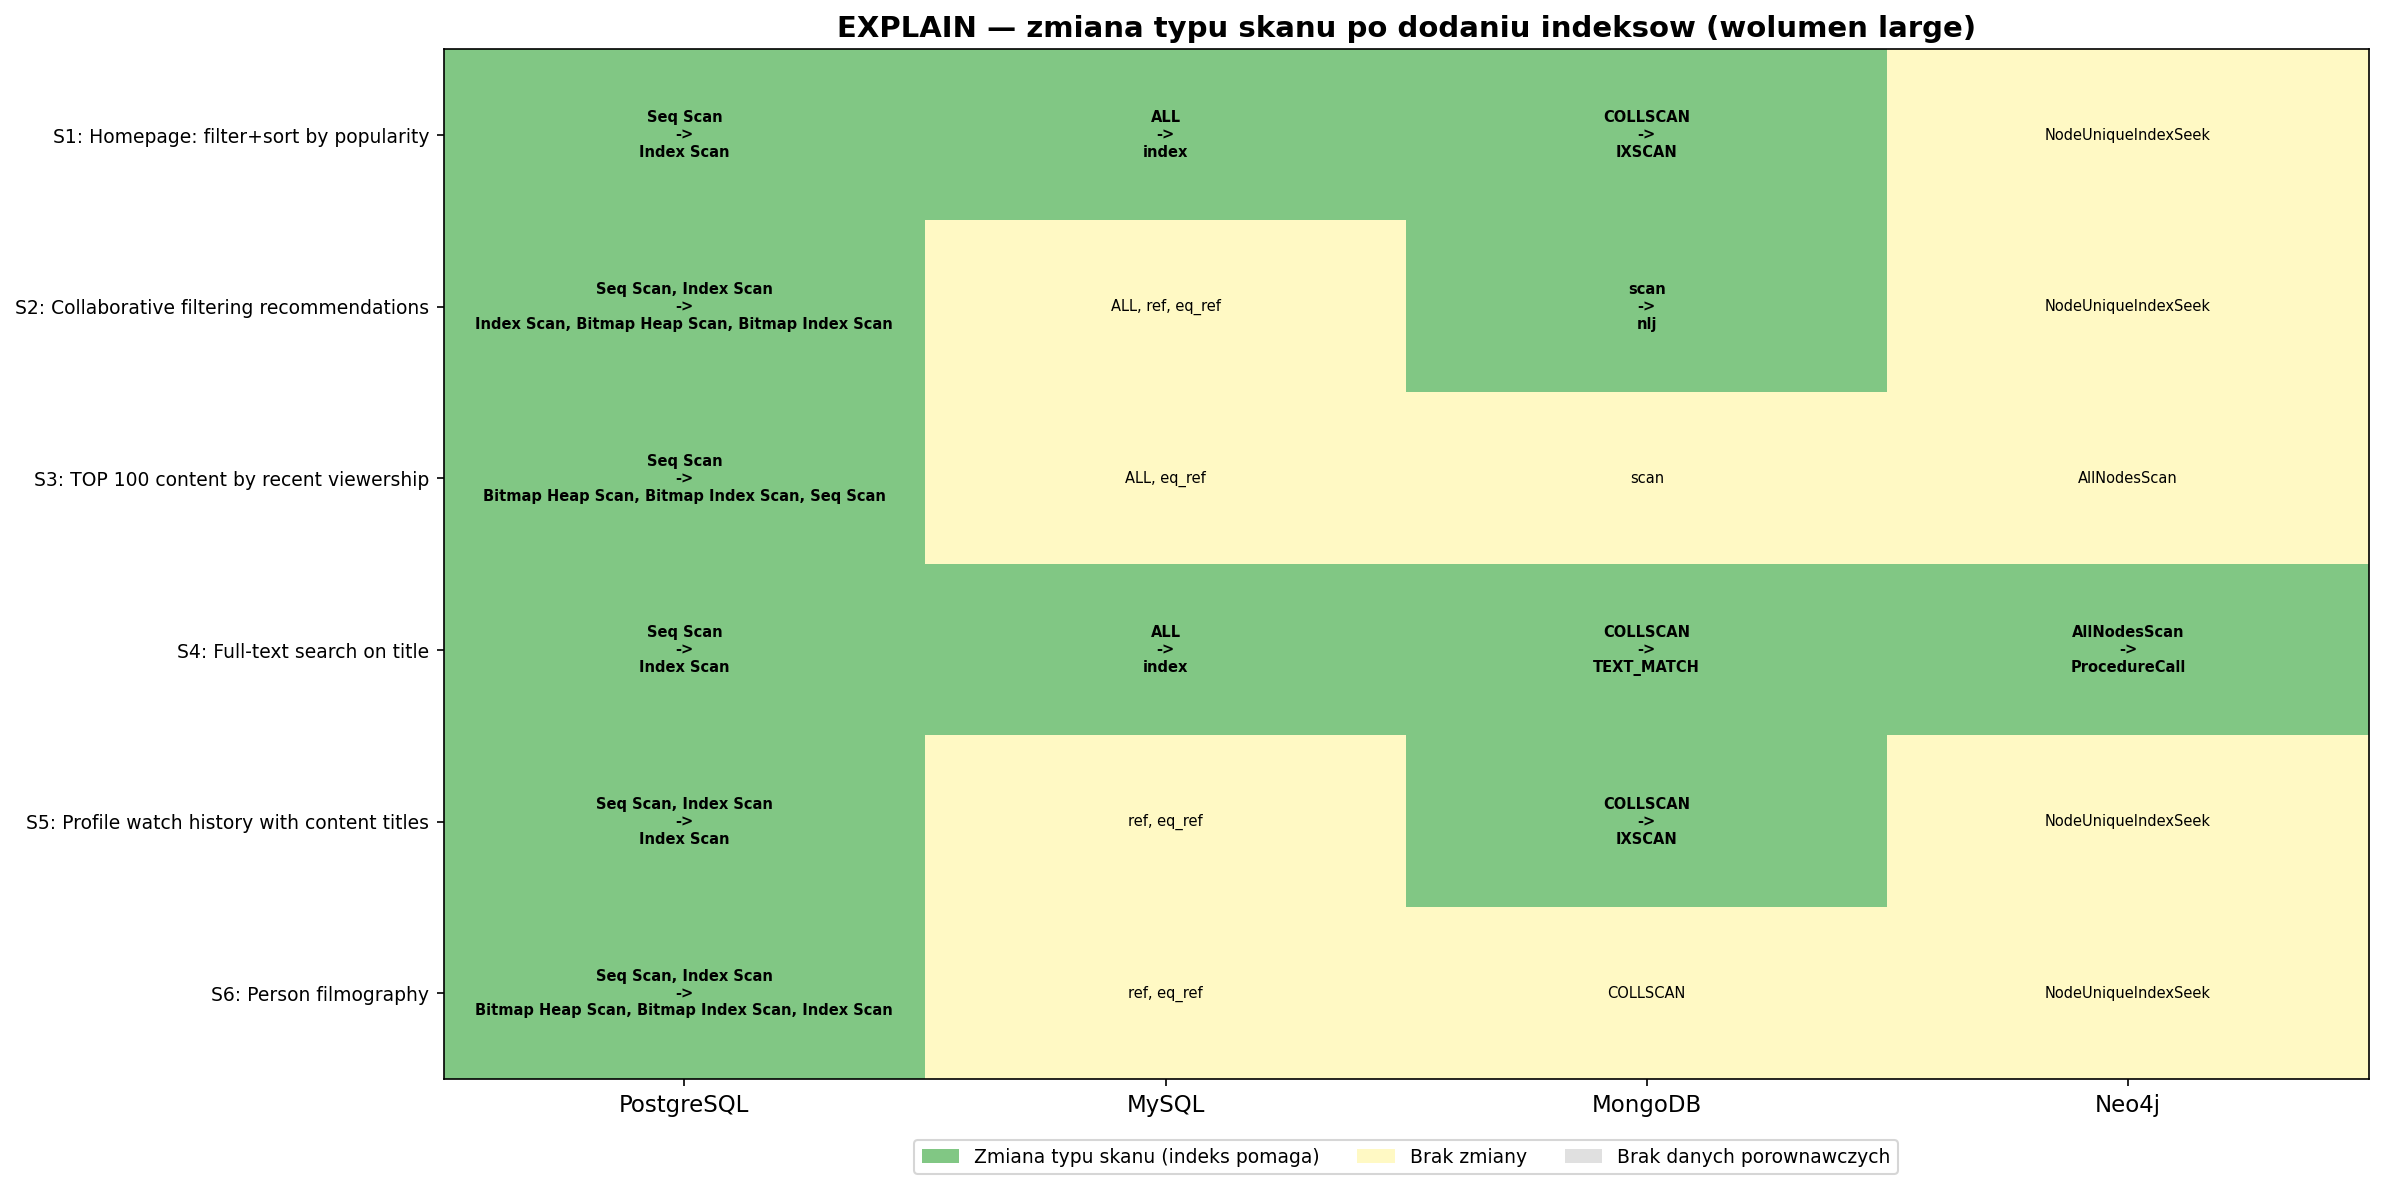
\includegraphics[width=1.0\textwidth]{charts/explain/explain_scan_changes_large.png}
    \caption{Zmiany typów skanów -- wolumen large, z indeksami}
\end{figure}

\begin{figure}[H]
    \centering
    
\includegraphics[width=1.0\textwidth]{charts/explain/explain_rows_examined_small.png}
    \caption{Liczba przejrzanych wierszy -- wolumen small, z indeksami}
\end{figure}

\begin{figure}[H]
    \centering
    
\includegraphics[width=1.0\textwidth]{charts/explain/explain_rows_examined_medium.png}
    \caption{Liczba przejrzanych wierszy -- wolumen medium, z indeksami}
\end{figure}

\begin{figure}[H]
    \centering
    
\includegraphics[width=1.0\textwidth]{charts/explain/explain_rows_examined_large.png}
    \caption{Liczba przejrzanych wierszy -- wolumen large, z indeksami}
\end{figure}

% -------------------------------------------------------

\subsection{Porównanie i wykresy}

\begin{figure}[H]
    \centering
    
\includegraphics[width=1.0\textwidth]{charts/explain/explain_exec_time_small.png}
    \caption{Czas wykonania zapytań SELECT -- wolumen small}
\end{figure}

\begin{figure}[H]
    \centering
    
\includegraphics[width=1.0\textwidth]{charts/explain/explain_exec_time_medium.png}
    \caption{Czas wykonania zapytań SELECT -- wolumen medium}
\end{figure}

\begin{figure}[H]
    \centering
    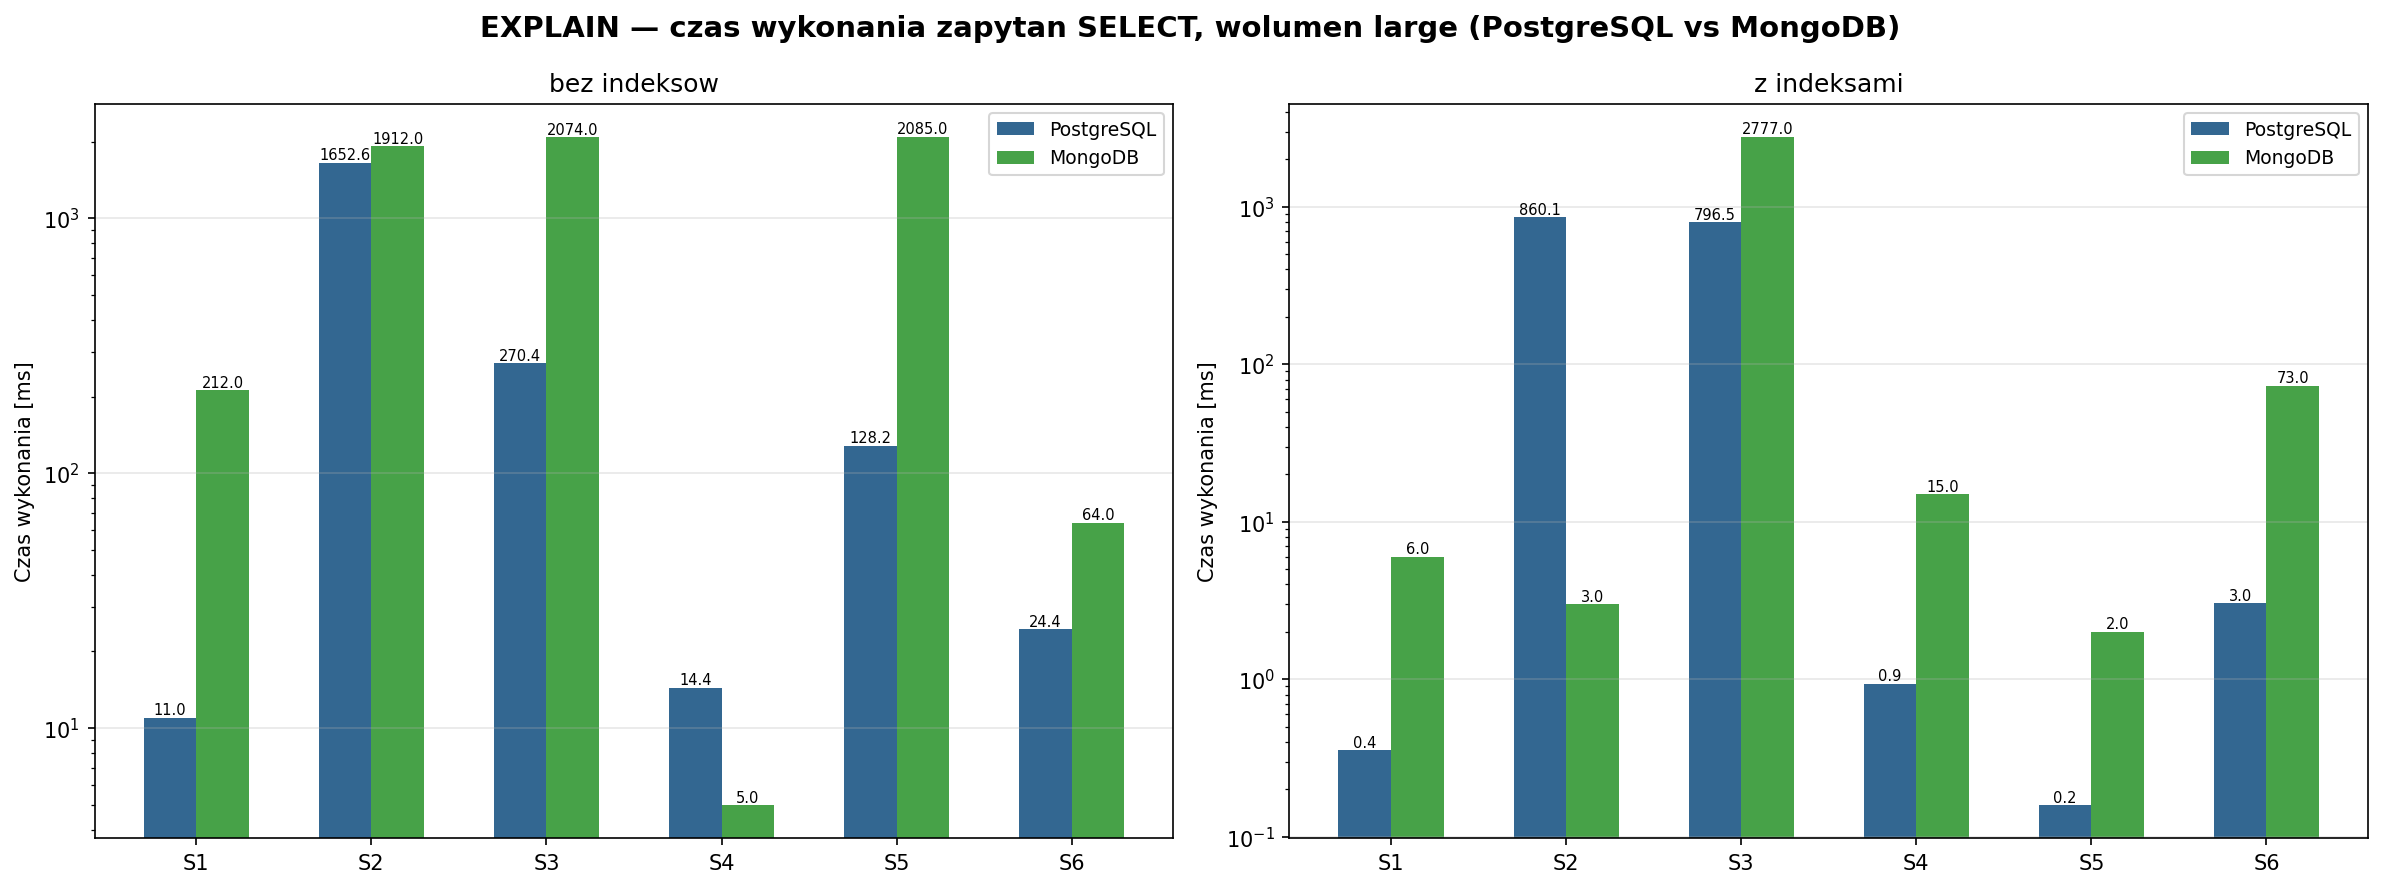
\includegraphics[width=1.0\textwidth]{charts/explain/explain_exec_time_large.png}
    \caption{Czas wykonania zapytań SELECT -- wolumen large}
\end{figure}